\chapter{Related Work}\label{ch:relatedWork}
% TODO: many certificate authorities also provide client email certificates:
% https://www.comodo.com/home/email-security/free-email-certificate.php
% https://www.digicert.com/client-certificates/
% https://www.globalsign.com/de-de/sichere-email/
% some even provide active directory integration / (aka managed PKI)
% however, none of them truly open-source, which should be a major requirement for all encryption (cf. Kerckhoffs' principle, cite schneier2007applied)
% and are priced at approximately 10€ per user, which turns out to be rather expensive for organizations such as TUM, with approx. 42k members.

A more recent project, providing encryption services is Let's Encrypt.
The Let's Encrypt system provides a way to automatically provide x509 certificates for client to server communication,
e.g.\ for HTTPS\@.
This system works via an Automatic Certificate Management Environment (ACME), which is specified in an IETF standard
working draft~\cite{letsencrypteacme}.

\begin{figure}
    \centering
    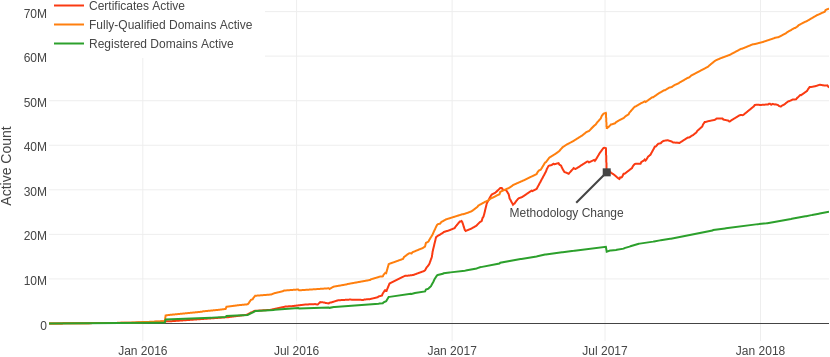
\includegraphics[width=\textwidth]{figures/letsencryptusers.png}
    \caption{Let's Encrypt Growth~\cite{letsencryptstats}}
    \label{fig:letsencrypt}
\end{figure}

This project is already immensely successful, providing over 50 Million active certificates, as of March 2018 (see
Figure~\ref{fig:letsencrypt})

However, this system is not intended for the general population, since the validation challenges aren't end-user
focused, but mostly for web servers.
X.509 certificates, as issued by Let's Encrypt can generally be used for email security with S/MIME\@.
Since this is not the focus of Let's encrypt, they also don't issue certificates, that would be usable for email
encryption.

More work about how email encryption certificates can be managed in a organization has been done by the TUM Secure
Email and User Certification Project~\cite{hauner2016interoperability, jagdish2016certservice, straub2016directoryservice, maier2015multidevice}
